% article Elsevier template - rax 01.05.2023
% main paper data
\def \ver {1.0}
\def \maintitle {A Prescriptive Simulation Optimization Framework for Capacity Planning in Healthcare System}
\def \shorttitle {Prescriptive framework for healthcare}
\def \shortauthors {Raúl Araneda M., Rodrigo A. Carrasco}
\def \keywordlist {Discrete Event Simulation \sep Derivative-Free Optimization \sep Healthcare}
\def \subject {subject}
\def \journalName {journal}

% ****************************************************************************
% Document Start
\documentclass[11pt]{elsarticle}
% **** packages ****
\usepackage[english]{babel}

\usepackage[utf8]{inputenc}
\usepackage{amsmath}
\usepackage{graphicx}
\usepackage{sidecap}
\usepackage{caption}
\usepackage{subfig}
\usepackage{transparent}
\usepackage{float}
\usepackage{amssymb}
\usepackage{nameref}
\usepackage{xargs}
\usepackage{natbib}
\usepackage{threeparttable}
\usepackage{booktabs}
\usepackage{tikz}
\usetikzlibrary{positioning}
\usetikzlibrary{arrows.meta}
\usetikzlibrary{shapes.geometric}

\usepackage[colorinlistoftodos,prependcaption,textsize=tiny]{todonotes}
\newcommandx{\rax}[2][1=]{\todo[linecolor=blue,backgroundcolor=blue!25,bordercolor=blue,#1]{#2}}

% add pdf hyper-ref layer
\input{rax_pdfsetup}

% ****************************************************************************
% **** page format ****
\usepackage{fullpage}

% size control
\usepackage[compact]{titlesec}

% page layout
\paperheight = 11in
\paperwidth = 8.5in
\textheight = 9.0in
\textwidth = 6.5in

% ****************************************************************************
% **** pieces and bits ****
\newtheorem{lemma}{Lemma}[section]
\newtheorem{theorem}{Theorem}[section]
\newtheorem{conjecture}{Conjecture}[section]
\newtheorem{corollary}{Corollary}[section]
\newtheorem{assumption}{Assumption}[section]

% ****************************************************************************
% **** rax commands/macros ****
\def \puc {Institute of Mathematical Engineering and Computation \& School of Engineering,\\ Pontificia Universidad Cat\'olica de Chile, Santiago, Chile}

% ****************************************************************************
% **** paper specific commands and macros ****
\usepackage{datetime}
\usepackage[overlay,absolute]{textpos}

\newcounter{buildyear}
\setcounter{buildyear}{\the\year}
\addtocounter{buildyear}{-2000}
\newcommand{\tdyear}{\arabic{buildyear}}
\newtimeformat{vtime}{\twodigit{\THEHOUR}\twodigit{\THEMINUTE}\twodigit{\THESECOND}}
\settimeformat{vtime}
\newcommand{\build}{\tdyear\twodigit{\the\month}\twodigit{\the\day}\currenttime}
\newcommand{\addbuild}{
	\begin{textblock*}{1in}(-5mm,\paperheight-25mm)
		\rotatebox{90}{\footnotesize {\color{gray!50!white} b.\build}}
	\end{textblock*}
}

\newcommand{\keywords}[1]{\par\noindent
	{\small{\bf Keywords}: #1}}

\journal{\journalName, v.\ver(\build)}

% ****************************************************************************

\begin{document}
%****************** Title ******************
\title{\maintitle}

\author{Raúl Araneda M.\corref{cor}}
\ead{rharaneda@uc.cl}
\address{School of Engineering,\\ Pontificia Universidad Cat\'olica de Chile, Santiago, Chile}

\author{Rodrigo A. Carrasco\corref{cor}}
\ead{rax@uc.cl}
\cortext[cor]{Corresponding author}

\address{\puc}

\begin{frontmatter}

\begin{abstract}

Chile's public specialty waiting lists exceed 2.9 million patients at the end of 2025, with mean waits above 260 days. In general, capacity parameters at ambulatory centers are set through an expert-driven process, without a formal optimization model. We build a discrete-event simulation (DES) of the minimally invasive gynecology (CMI) pathway at CRS Cordillera, Santiago, validate it against operational data (Mann--Whitney $U=865{,}529$, $p=0.056$), and use it as a black-box evaluator to benchmark seven black-box optimizers under common random numbers.

Every method significantly reduces average time in system (ATS) by 27--34\% relative to the incumbent policy while simultaneously increasing patients served, a strict Pareto improvement. The best mean ATS is achieved by SPSA (174.5 days), but SPSA treats integer decision variables as continuous and rounds post-hoc, and its convergence guarantee assumes constant noise variance, a condition the DES evaluator violates structurally. SMAC-SK, which replaces SMAC's default surrogate with a stochastic-kriging model that explicitly separates simulation noise from metamodel uncertainty, achieves a statistically indistinguishable ATS (176.9 days, $p=0.08$), handles mixed-integer variables natively, and produces the tightest confidence interval among competitive methods ($\sigma=4.7$ vs.\ $6.3$ for SPSA).

\end{abstract}

\begin{keyword}
\keywordlist
\end{keyword}
\end{frontmatter}

\section{Introduction}

Chile's public health system had 2{,}978{,}427 patients on specialty and surgery waiting lists at the end of 2025, with a mean waiting time of 266 days for specialist care \citep{MINSAL2025}. The problem is not purely one of supply: \citet{Martinez2019} show that even patients with non-prioritized conditions face increased mortality risk as waiting times grow, and OECD evidence points to scheduling quality, administrative follow-up, and prioritization tools as independent drivers of wait times \citep{OECD2020,OECD2025}.

Discrete-event simulation (DES) has become the standard tool for studying these systems \citep{Law2015,MonksHarper2025}. A DES model can replicate the patient pathway in detail: stochastic arrivals, triage rules, multiple care stages, and no-shows, producing estimates of waiting time under a given configuration. What it cannot do on its own is identify which configuration to use. For that, DES must be coupled with an optimizer.

The DES evaluator is a black box: no gradient is available, each evaluation is expensive, and output variance is not constant across the decision space. Near-capacity configurations are noisier than configurations with slack, a property known as structural heteroscedasticity. Most DFO and SO methods with formal convergence guarantees assume constant noise variance \citep{Conn2009,Amaran2016,Shashaani2018}; methods that do model heteroscedastic variance lack either mixed-integer support or convergence results, a gap we discuss in Section~\ref{sec:litreview}.

We model the CMI (minimally invasive gynecology) patient pathway at CRS Cordillera, a public ambulatory referral center in Santiago, and propose SMAC-SK as the configuration-search tool. SMAC-SK replaces SMAC's default surrogate \citep{Hutter2011,Lindauer2022} with a stochastic-kriging model \citep{Ankenman2010} that separates simulation noise from metamodel uncertainty, letting the acquisition function distinguish configurations that need more replications from configurations that need more exploration. We benchmark SMAC-SK against six other black-box optimizers on the validated DES evaluator.

The main finding: every optimizer significantly outperforms the incumbent policy, reducing ATS by 27--34\% while simultaneously increasing patients served. SMAC-SK is the recommended method, not because it achieves the lowest mean ATS (SPSA does, by a statistically non-significant margin), but because it handles mixed-integer decision variables natively, models the evaluator's heteroscedasticity, and produces the tightest confidence interval.


\section{Our contributions}

The central contribution of this work is applied: we show that SMAC-SK, obtained by coupling the SMAC sequential model-based configuration framework \citep{Lindauer2022,Hutter2011} with a stochastic-kriging surrogate \citep{Ankenman2010} in place of its default random-forest or Gaussian-process surrogates, is a practical and effective tool for improving capacity planning for CMI at CRS Cordillera, and we recommend it as the configuration-search method of choice for this class of problem. SMAC-SK is, to our knowledge, a combination not previously reported in the literature: the stochastic-kriging surrogate explicitly decomposes the predicted response into intrinsic simulation variance and extrinsic metamodel uncertainty.

Beyond this central result, the work contributes: first, a statistically validated DES model of the CMI patient pathway at CRS Cordillera. Second, a controlled benchmark of seven black-box optimizers, including SMAC-SK, under common random numbers, showing that every algorithmically optimized configuration strictly Pareto-dominates the expert-driven policy currently in use. Third, an empirical characterization of the trade-off between convergence guarantees and achieved performance: the only benchmarked method with a formal almost-sure convergence guarantee (ASTRO-DF) is also the method that performs worst on this evaluator, which motivates further methodological work on DFO methods that retain convergence guarantees under structural heteroscedasticity.


\section{Case Study}

CRS Cordillera is a public ambulatory referral center serving Macul and Peñalolén in Santiago, with more than 30{,}000 consultations in 2025. Gynecology is the largest specialty by volume, around 30\% of activity, with 2{,}419 patients on the active waiting list at the time of data collection, a mean wait of 205 days for a first consultation, and a recorded maximum of 1{,}164 days.

This work focuses on CMI, the subspecialty covering endometriosis, uterine fibroids, and pelvic floor disorders. CMI held 318 active cases and a mean first-consultation wait of 81 days, the fifth-largest subspecialty list at the center. Demand arrives exclusively through referrals from primary care.

Patients enter the pathway with a clinical priority (high, medium, or low) and join the first-consultation waiting list. About 20\% pass through a pre-examination step before their first consultation; the rest proceed directly. After the first consultation, 67\% are scheduled for a follow-up, 5\% require pre-surgical assessment, and the remainder move to the surgical waiting list. Among surgical patients, roughly 30\% carry an endometriosis diagnosis and may need further follow-up. Losses occur at every transition: 17\% no-show, 32\% administrative blocking, 15\% non-contactability. See Figure~\ref{fig:pathway}.

Slot capacity is set through an expert-driven process, weekly counts for first and follow-up consultations; diagnostic resource allocation (laboratory and ultrasound); midwife staffing; and blocking and non-contactability targets, without a formal optimization model. The 12 decision variables that define a configuration are listed in Table~\ref{tab:decisionvars}, and the stochastic inputs of the DES model are described in Table~\ref{tab:distributions}.

\begin{figure}[H]
\centering
\includegraphics[width=\textwidth]{macro.png}
\caption{CMI patient pathway at CRS Cordillera.}
\label{fig:pathway}
\end{figure}

\begin{table}[H]
\centering
\caption{Decision variables for the CMI capacity configuration problem.}
\label{tab:decisionvars}
\small
\begin{tabular}{@{}clccc@{}}
\toprule
\# & Variable & Type & Base Line & Range \\
\midrule
1 & First-consult slots per week        & Integer    & 16   & [8, 30]      \\
2 & Post-control slots per week         & Integer    & 40   & [20, 60]     \\
3 & Lab slots per week (UGD)            & Integer    & 10   & [5, 20]      \\
4 & Ultrasound slots per week (UGD)     & Integer    & 8    & [4, 16]      \\
5 & Ultrasound slots per week (midwife) & Integer    & 6    & [3, 12]      \\
6 & Number of midwives                  & Integer    & 2    & [1, 4]       \\
7 & Number of UGD agents                & Integer    & 3    & [1, 6]       \\
8 & Scheduling lead time                & Integer    & 5    & [1, 10] days \\
\midrule
9  & First-consult blocking rate        & Continuous & 0.32 & [0.05, 0.50] \\
10 & Empty consult rate                 & Continuous & 0.17 & [0.05, 0.35] \\
11 & Non-contactability rate            & Continuous & 0.15 & [0.05, 0.30] \\
12 & Post-control blocking rate         & Continuous & 0.20 & [0.05, 0.40] \\
\bottomrule
\end{tabular}
\end{table}

\begin{table}[H]
\centering
\caption{Stochastic inputs of the DES model.}
\label{tab:distributions}
\begin{threeparttable}
\small
\begin{tabular}{@{}llll@{}}
\toprule
Component & Distribution & Parameters & Units \\
\midrule
\multicolumn{4}{@{}l}{\textit{Arrival \& capacity}} \\[2pt]
Daily patient arrivals
  & $\mathrm{NegBin}(n,\,p)$\tnote{$\dagger$}
  & $n=8.99,\; p=0.716$
  & patients/day \\
Weekly first-consult capacity\tnote{$b$}
  & $\mathrm{Gamma}(\alpha,\,\beta)$
  & $\alpha=8.37,\; \beta=1.77$
  & slots/week \\
Weekly post-control capacity\tnote{$b$}
  & $3.5 + 26.8\cdot\mathrm{Beta}(\alpha,\,\beta)$
  & $\alpha=0.945,\; \beta=1.63$
  & hours/week \\
\midrule
\multicolumn{4}{@{}l}{\textit{Initial backlog - first consult\tnote{$b$}}} \\[2pt]
Prior wait, HIGH priority
  & $7 + 274\cdot\mathrm{Beta}(\alpha,\,\beta)$
  & $\alpha=0.947,\; \beta=1.37$
  & days \\
Prior wait, MID priority
  & $7 + 238\cdot\mathrm{Beta}(\alpha,\,\beta)$
  & $\alpha=0.747,\; \beta=0.899$
  & days \\
Prior wait, LOW priority
  & $\mathrm{Uniform}(a,\,b)$
  & $a=42,\; b=242$
  & days \\
\midrule
\multicolumn{4}{@{}l}{\textit{Initial backlog - post-consultation\tnote{$b$}}} \\[2pt]
Prior wait, HIGH priority
  & $a + (b-a)\cdot\mathrm{Beta}(\alpha,\,\beta)$
  & $[7,\,544],\;\mu=126.0$
  & days \\
Prior wait, MID priority
  & $a + (b-a)\cdot\mathrm{Beta}(\alpha,\,\beta)$
  & $[7,\,684],\;\mu=114.0$
  & days \\
Prior wait, LOW priority
  & $a + (b-a)\cdot\mathrm{Beta}(\alpha,\,\beta)$
  & $[14,\,643],\;\mu=132.7$
  & days \\
\midrule
\multicolumn{4}{@{}l}{\textit{Pre-booking local adjustment (by priority)}} \\[2pt]
HIGH & $\mathrm{Uniform}(a,\,b)$ & $a=0.5,\; b=2.0$ & workdays \\
MID  & $\mathrm{Uniform}(a,\,b)$ & $a=1.0,\; b=4.0$ & workdays \\
LOW  & $\mathrm{Uniform}(a,\,b)$ & $a=1.0,\; b=5.0$ & workdays \\
\midrule
\multicolumn{4}{@{}l}{\textit{Procedure lead times}} \\[2pt]
Midwife review duration
  & $\mathrm{Uniform}(a,\,b)$ & $a=20,\; b=30$  & min  \\
Anesthesiologist scheduling lead
  & $\mathrm{Uniform}(a,\,b)$ & $a=21,\; b=30$  & days \\
Surgery scheduling lead (CRS Cordillera)
  & $\mathrm{Uniform}(a,\,b)$ & $a=60,\; b=90$  & days \\
Resident post-op review request
  & $\mathrm{Uniform}(a,\,b)$ & $a=4,\;  b=6$   & days \\
\bottomrule
\end{tabular}
\begin{tablenotes}
\footnotesize
\item[$\dagger$] Left-truncated at $k \geq 1$; zero counts are redrawn.
      Mean daily rate $= n(1-p)/p = 3.57$ patients/day, validated
      against CMI records ($n=52$ weeks, $\hat{\mu}=3.66$/day;
      NegBin MLE: $\chi^2=4.83$, $p=0.185$).
\item[$b$] Beta parameters fitted to historical waiting-list records;
      all distributions validated against operational data prior to model deployment.
\end{tablenotes}
\end{threeparttable}
\end{table}


\section{Problem Definition}
\label{sec:problem}

We seek a capacity configuration $x = (x_1,\dots,x_{12}) \in \mathcal{X}$ that minimizes ATS, the mean number of days from referral to discharge, for CMI patients at CRS Cordillera. The decision space is mixed-integer, $\mathcal{X} \subset \mathbb{Z}^{8} \times \mathbb{R}^{4}$, with eight integer variables (slot counts, staffing levels, scheduling lead time) and four continuous variables (blocking and loss rates), all subject to box constraints $\ell \le x \le u$ as listed in Table~\ref{tab:decisionvars}. Formally:

\begin{equation}
\min_{x \in \mathcal{X}} \; f(x) = \mathbb{E}\big[\mathrm{ATS}(x;\omega)\big],
\label{eq:problem}
\end{equation}

where $\omega$ captures simulation randomness (arrivals, weekly capacity, initial backlog). Because $f(x)$ has no closed form, each evaluation requires a full DES run and returns only the noisy estimate $\mathrm{ATS}(x;\omega)$.

A feature of this evaluator that shapes the choice of optimizer is that output variance $\sigma^2(x)$ is not constant across $\mathcal{X}$. Configurations near capacity saturation, where queues are long and sensitive to small perturbations, are substantially noisier than configurations with slack. Figure~\ref{fig:pathway} illustrates where this arises structurally: blocking, no-show, and non-contactability rates interact with slot counts in a way that makes the queue regime, and therefore the noise level, a function of $x$. This heteroscedasticity invalidates the constant-variance assumption that underlies the convergence guarantees of most DFO and SO methods, and motivates an optimizer that can estimate $\sigma^2(x)$ locally.


\section{Literature Review}
\label{sec:litreview}

DES has become the standard tool for modeling patient pathways, waiting times, and scheduling rules in health systems \citep{MonksHarper2025,Law2015}. Its strength is fidelity: a DES model can capture stochastic arrivals, multiple care stages, and competing resources in detail. Its limitation is that it is evaluative; it tells you how a configuration performs, not which configuration to choose. Coupling DES with an optimizer is the natural extension, and it is what SO \citep{Amaran2016} and DFO \citep{Conn2009} are designed for when the evaluator is expensive and gradient-free.

ASTRO-DF \citep{Shashaani2018} constructs local polynomial models from Monte Carlo estimates within a trust-region framework and proves almost-sure convergence to first-order stationary points; \citet{HaShashaani2025} sharpen this to an iteration complexity of $\mathcal{O}(\varepsilon^{-2})$ almost surely. Both results assume variance is bounded and uniform across the trust region. SPSA \citep{Spall1992} takes a different route: it estimates the gradient by perturbing all variables simultaneously along a single random direction, requiring only two evaluations per iteration regardless of dimension. It is cheap and simple, but it builds no model of the landscape, makes no use of variance structure, and converges almost surely only under conditions on step-size and perturbation sequences that assume homoscedastic noise.

SMAC3 \citep{Lindauer2022} wraps a random-forest or Gaussian-process surrogate inside a sequential model-based configuration loop. Random forests handle mixed-integer and categorical variables natively; the Gaussian-process variant does not. Both assume homogeneous noise across the design space. Stochastic kriging \citep{Ankenman2010} is the first surrogate designed explicitly for heteroscedastic simulation output: it decomposes predicted variance into an intrinsic component (simulation noise, estimated from replications) and an extrinsic component (metamodel uncertainty). \citet{Ankenman2010} prove consistency of the predictor but do not embed it in a mixed-integer optimizer. Complementary work on sequential design for replicated stochastic simulation \citep{Binois2019} and the \texttt{hetGP} software \citep{BinoisGramacy2021hetGP,Binois2018} operationalize this decomposition outside the mixed-integer setting. Gaussian-process surrogates have also been incorporated into trust-region methods: \citet{Menhorn2017} use them to mitigate noise in a constrained framework without modeling point-dependent variance, and \citet{Shukla2020} establish global convergence for a GP-based trust-region method under a homoscedasticity assumption. \citet{Scott2011} propose the knowledge gradient for continuous parameters (KGCP), which selects the next evaluation by expected information value; it admits a point-dependent noise variance but assumes it is known and treats the decision space as continuous.

COMPASS \citep{HongNelson2006} proves almost-sure convergence to a local optimum over integer-ordered spaces through iterative refinement of a promising region with a replication-allocation rule that controls estimation error. R-SPLINE \citep{WangRSPLINE2013} extends this to the mixed-integer case, combining a continuous relaxation with neighborhood enumeration and establishing almost-sure convergence via a retrospective growing-budget scheme. Both assume constant variance. For deterministic evaluators, \citet{NewbyAli2015} and \citet{Torres2024MITR} establish convergence to mixed-integer stationary points within trust-region frameworks; NOMAD \citep{LeDigabel2011}, implementing mesh-adaptive direct search \citep{Audet2006}, guarantees convergence to Clarke-stationary points over mixed-variable domains without a surrogate; and \citet{Bliek2021} propose a mixed-variable surrogate that satisfies integer constraints natively. None is designed for a stochastic, heteroscedastic evaluator.

Simulated annealing, genetic algorithms, tabu search, and commercial packages such as OptQuest \citep{Laguna2003} are the most common tools in applied healthcare SO \citep{Wang2023}. Convergence results exist for simulated annealing under specific cooling schedules \citep{Hajek1988,Alrefaei1999}, but they assume bounded, homoscedastic noise.

Each line of work solves part of the problem. Stochastic kriging models heteroscedastic variance but has not been embedded in a mixed-integer optimizer. SMAC handles mixed-integer spaces but assumes homoscedastic noise. Methods with formal convergence guarantees for integer or mixed-integer spaces assume constant variance and do not tie replication allocation to local variance estimates. To our knowledge, no reported method combines all four conditions simultaneously: a stochastic black-box evaluator with structural heteroscedasticity, mixed-integer decision variables, an adaptive replication rule tied to local variance, and formal convergence guarantees. The difficulty is not merely that these conditions co-occur; whether $\sigma^2(x)$ changes discontinuously across integer boundaries of the decision space is an open theoretical question that affects convergence analysis directly.


\section{Method}
\label{sec:method}

The study proceeds in two stages. First, we build and validate a DES of the CMI pathway at CRS Cordillera. Second, we use the validated evaluator to benchmark seven black-box optimizers under common random numbers (CRN).

\subsection{DES Model and Validation}

The DES model is implemented in SimPy and covers the full CMI pathway from referral through first consultation, follow-up, and surgical or post-surgical care, using the stochastic inputs described in Table~\ref{tab:distributions}. Each run covers a 52-week horizon. Initial waiting-list backlogs are seeded from the calibrated distributions, reproducing the observed queue state at the start of the simulation rather than relying on a warm-up period. The primary output is ATS. Model fidelity against the September~2025 waiting-list extract is reported in Section~\ref{sec:results}.

\subsection{Benchmark Design}

The validated DES evaluator is coupled to seven optimizers, each run for $S = 15$ independent macro-seeds with $n_r = 3$ DES replications per candidate evaluation: SPSA \citep{Spall1992}; ASTRO-DF \citep{Shashaani2018}; two SMAC configurations with Gaussian-process (SMAC-GP+EI) and random-forest (SMAC-RF) surrogates \citep{Lindauer2022}; and three stochastic-kriging-based methods (SMAC-SK, SK-Adaptive, SK-KGCP \citep{Scott2011}). All methods are compared on ATS and patients served against the incumbent policy under a unified budget of $B = 150$ simulator evaluations per macro-replication ($S \times B = 2{,}250$ simulator calls per method). Table~\ref{tab:methods} summarises each method's surrogate type, variance modelling, mixed-integer support, and convergence guarantees.

\begin{table}[H]
\centering
\caption{Benchmarked methods, surrogate type, and variable handling.}
\label{tab:methods}
\begin{threeparttable}
\small
\begin{tabular}{@{}llccc@{}}
\toprule
Method & Surrogate & Models $\sigma^2(x)$ & Mixed-integer & Convergence \\
\midrule
SPSA         & ---               & --           & $\checkmark^\dagger$ & a.s.$^{*}$ \\
ASTRO-DF     & Linear/quadratic  & --           & $\checkmark^\dagger$ & a.s.$^{*}$ \\
SMAC-GP+EI   & Gaussian process  & --           & $\checkmark^\dagger$ & None \\
SMAC-RF      & Random forest     & Partial      & $\checkmark$         & None \\
SMAC-SK      & Stochastic kriging& $\checkmark$ & $\checkmark$         & None \\
SK-Adaptive  & Stochastic kriging& $\checkmark$ & $\checkmark^\dagger$ & None \\
SK-KGCP      & Stochastic kriging& $\checkmark$ & $\checkmark^\dagger$ & None \\
\bottomrule
\end{tabular}
\begin{tablenotes}
\footnotesize
\item[$*$] Convergence assumes homoscedastic noise --- not satisfied by the CMI DES evaluator.
\item[$\dagger$] Integers handled via continuous relaxation and rounding, not natively.
\end{tablenotes}
\end{threeparttable}
\end{table}

\subsection{SMAC-SK}
\label{sec:smacsk}

SMAC-SK replaces SMAC's default surrogate with a stochastic-kriging (SK) model \citep{Ankenman2010} inside SMAC's sequential model-based configuration loop \citep{Hutter2011,Lindauer2022}. For a configuration $x$ evaluated with $r(x)$ replications, SK decomposes the predicted response as
\begin{equation}
\hat{Y}(x) = \mu(x) + M(x) + \varepsilon(x),
\qquad
\mathrm{Var}[\varepsilon(x)] = \sigma^2_\varepsilon(x),
\qquad
\mathrm{Var}[M(x)] = \sigma^2_M(x),
\label{eq:sk}
\end{equation}
where $\mu(x)$ is the trend, $M(x)$ captures extrinsic metamodel uncertainty via a Gaussian process, and $\varepsilon(x)$ captures intrinsic simulation noise estimated from the sample variance of the $r(x)$ replications at $x$. A random forest conflates both sources into a single predictive variance; a standard Gaussian process assumes $\sigma^2_\varepsilon(x)$ is constant across the space. Neither distinction is available without replication-aware noise modelling.

Figure~\ref{fig:smacsk} shows the resulting loop. The SK surrogate is refit after each evaluation; the EI acquisition function searches the mixed-integer neighborhood trading off low $\mu(x)$ against high $\sigma^2_M(x)$; and an adaptive-replication rule decides whether to run additional replications at the current configuration or move to a new one. The loop terminates when the budget is exhausted, returning $x^{*} = \arg\min \hat{\mu}(x)$.

\begin{figure}[H]
\centering
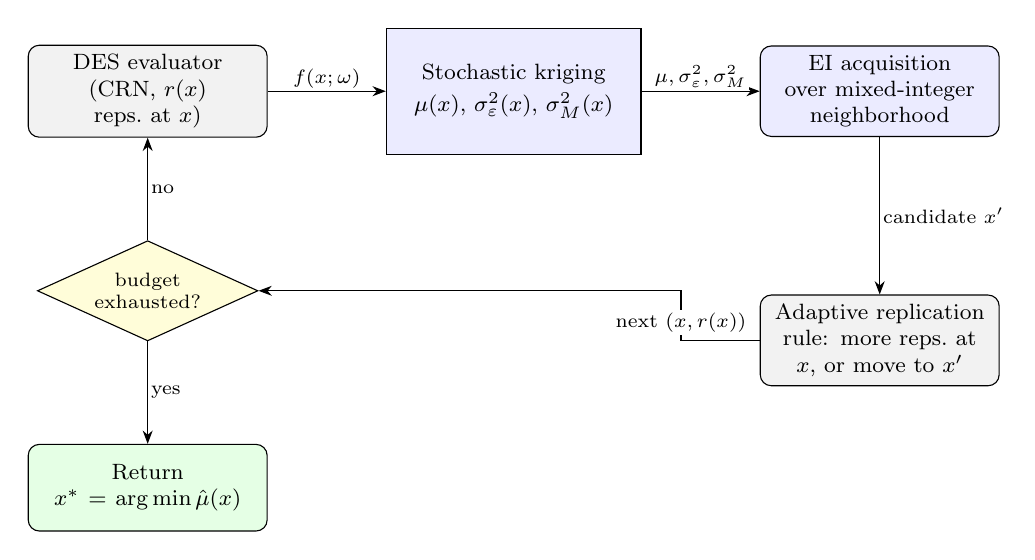
\begin{tikzpicture}[
  node distance=13mm and 15mm,
  box/.style={draw, rounded corners, align=center, minimum height=1.1cm,
              minimum width=2.9cm, text width=2.8cm, font=\footnotesize},
  sk/.style={draw, align=center, minimum height=1.6cm,
             minimum width=3.1cm, text width=3.0cm, font=\footnotesize},
  dec/.style={draw, diamond, aspect=2.2, align=center,
              font=\scriptsize, inner sep=2pt},
  lbl/.style={font=\scriptsize, align=center, fill=white, inner sep=1pt},
  >=Stealth
]
  \node[box, fill=gray!10] (des)
        {DES evaluator\\(CRN, $r(x)$ reps.\ at $x$)};
  \node[sk,  fill=blue!8,  right=of des] (sk)
        {Stochastic kriging\\[2pt]
         $\mu(x),\,\sigma^2_\varepsilon(x),\,\sigma^2_M(x)$};
  \node[box, fill=blue!8,  right=of sk]  (ei)
        {EI acquisition over mixed-integer neighborhood};
  \node[box, fill=gray!10, below=20mm of ei] (rep)
        {Adaptive replication rule: more reps.\ at $x$,
         or move to $x'$};
  \node[dec, fill=yellow!15, below=13mm of des] (dec)
        {budget\\exhausted?};
  \node[box, fill=green!10, below=13mm of dec, text width=2.8cm] (out)
        {Return $x^{*}=\arg\min\hat{\mu}(x)$};

  \draw[->] (des) -- node[lbl,above]{$f(x;\omega)$} (sk);
  \draw[->] (sk)  -- node[lbl,above]{$\mu,\sigma^2_\varepsilon,\sigma^2_M$} (ei);
  \draw[->] (ei)  -- node[lbl,right]{candidate $x'$} (rep);
  \draw[->] (rep.west) -- ++(-10mm,0)
              |- node[lbl,pos=0.05,above]{next $(x,r(x))$} (dec.east);
  \draw[->] (dec) -- node[lbl,right]{no}  (des);
  \draw[->] (dec) -- node[lbl,right]{yes} (out);
\end{tikzpicture}
\caption{The SMAC-SK optimisation loop.}
\label{fig:smacsk}
\end{figure}


\section{Results}
\label{sec:results}

\subsection{DES Model Validation}

To assess whether the calibrated model reproduces the current waiting-list state, simulated ATS distributions were compared against the September~2025 extract for CRS Cordillera using a two-sample Mann--Whitney test. The test does not reject distributional equivalence ($U = 865{,}529$, $p = 0.056$; Table~\ref{tab:validation}, Appendix~\ref{app:validation}), supporting use of the DES as a black-box evaluator for the optimisation experiment.

\subsection{Benchmark Results}

Table~\ref{tab:results} reports ATS and patients served for the incumbent policy and for the best configuration found by each optimizer ($n = 18$ replications; Appendix~\ref{app:replication}). Every algorithm reduces ATS relative to the incumbent (Wilcoxon signed-rank test, $p \ll 0.001$ in all cases) while simultaneously increasing patients served, a strict Pareto improvement with no wait-time/throughput trade-off (Figure~\ref{fig:Pareto}).

\begin{table}[H]
\centering
\caption{Benchmark results: ATS and patients served relative to the incumbent policy
         ($n = 18$ replications; Appendix~\ref{app:replication}).}
\label{tab:results}
\begin{threeparttable}
\begin{tabular}{@{}lcccc@{}}
\toprule
Method & ATS $\mu\pm\sigma$ (days) & 95\% CI & Served
       & $\Delta$ vs.\ Incumbent (days) \\
\midrule
Incumbent    & $263.0\pm7.1$ & [259.7, 266.2] & 1{,}148 & --- \\
\midrule
SPSA         & $174.5\pm6.3$ & [172.7, 176.2] & 2{,}216 & $-88.5$ \\
SMAC-GP+EI   & $174.9\pm7.0$ & [173.0, 176.9] & 1{,}895 & $-88.0$ \\
SK-Adaptive  & $176.6\pm5.9$ & [174.9, 178.2] & 2{,}206 & $-86.4$ \\
\textbf{SMAC-SK} & $\mathbf{176.9\pm4.7}$ & \textbf{[175.6, 178.2]}
             & \textbf{2{,}179} & $\mathbf{-86.0}$ \\
SMAC-RF      & $182.1\pm5.3$ & [180.6, 183.5] & 1{,}807 & $-80.9$ \\
SK-KGCP      & $192.0\pm6.2$ & [190.3, 193.7] & 1{,}836 & $-71.0$ \\
ASTRO-DF     & $218.6\pm0.5$ & [218.4, 218.9] & 2{,}103 & $-44.3$ \\
\bottomrule
\end{tabular}
\begin{tablenotes}
\footnotesize
\item All algorithms reduce ATS relative to Incumbent
      (Wilcoxon signed-rank, $p\ll0.001$).
\end{tablenotes}
\end{threeparttable}
\end{table}

SPSA attains the lowest ATS point estimate ($174.5$ days, $-33.7\%$ vs.\ Incumbent) and the highest patient throughput ($2{,}216$). SMAC-SK reaches a comparable point estimate ($176.9$ days, $-32.7\%$) with the tightest confidence interval among all methods and the lowest run-to-run standard deviation among competitive methods ($\sigma = 4.7$ days), consistent with its replication-aware noise model reducing metamodel uncertainty near the optimum.

ASTRO-DF, the only benchmarked method with a formal almost-sure convergence guarantee, yields the highest residual ATS ($218.6$ days, $-16.9\%$). Its near-zero run-to-run variance ($\sigma = 0.5$ days) indicates stable but conservative behaviour: the adaptive-sampling criterion accumulates replications rather than exploring the space, a response consistent with the structural heteroscedasticity of the DES evaluator violating the homoscedastic noise assumption underlying its convergence proof.

\begin{figure}[H]
\centering
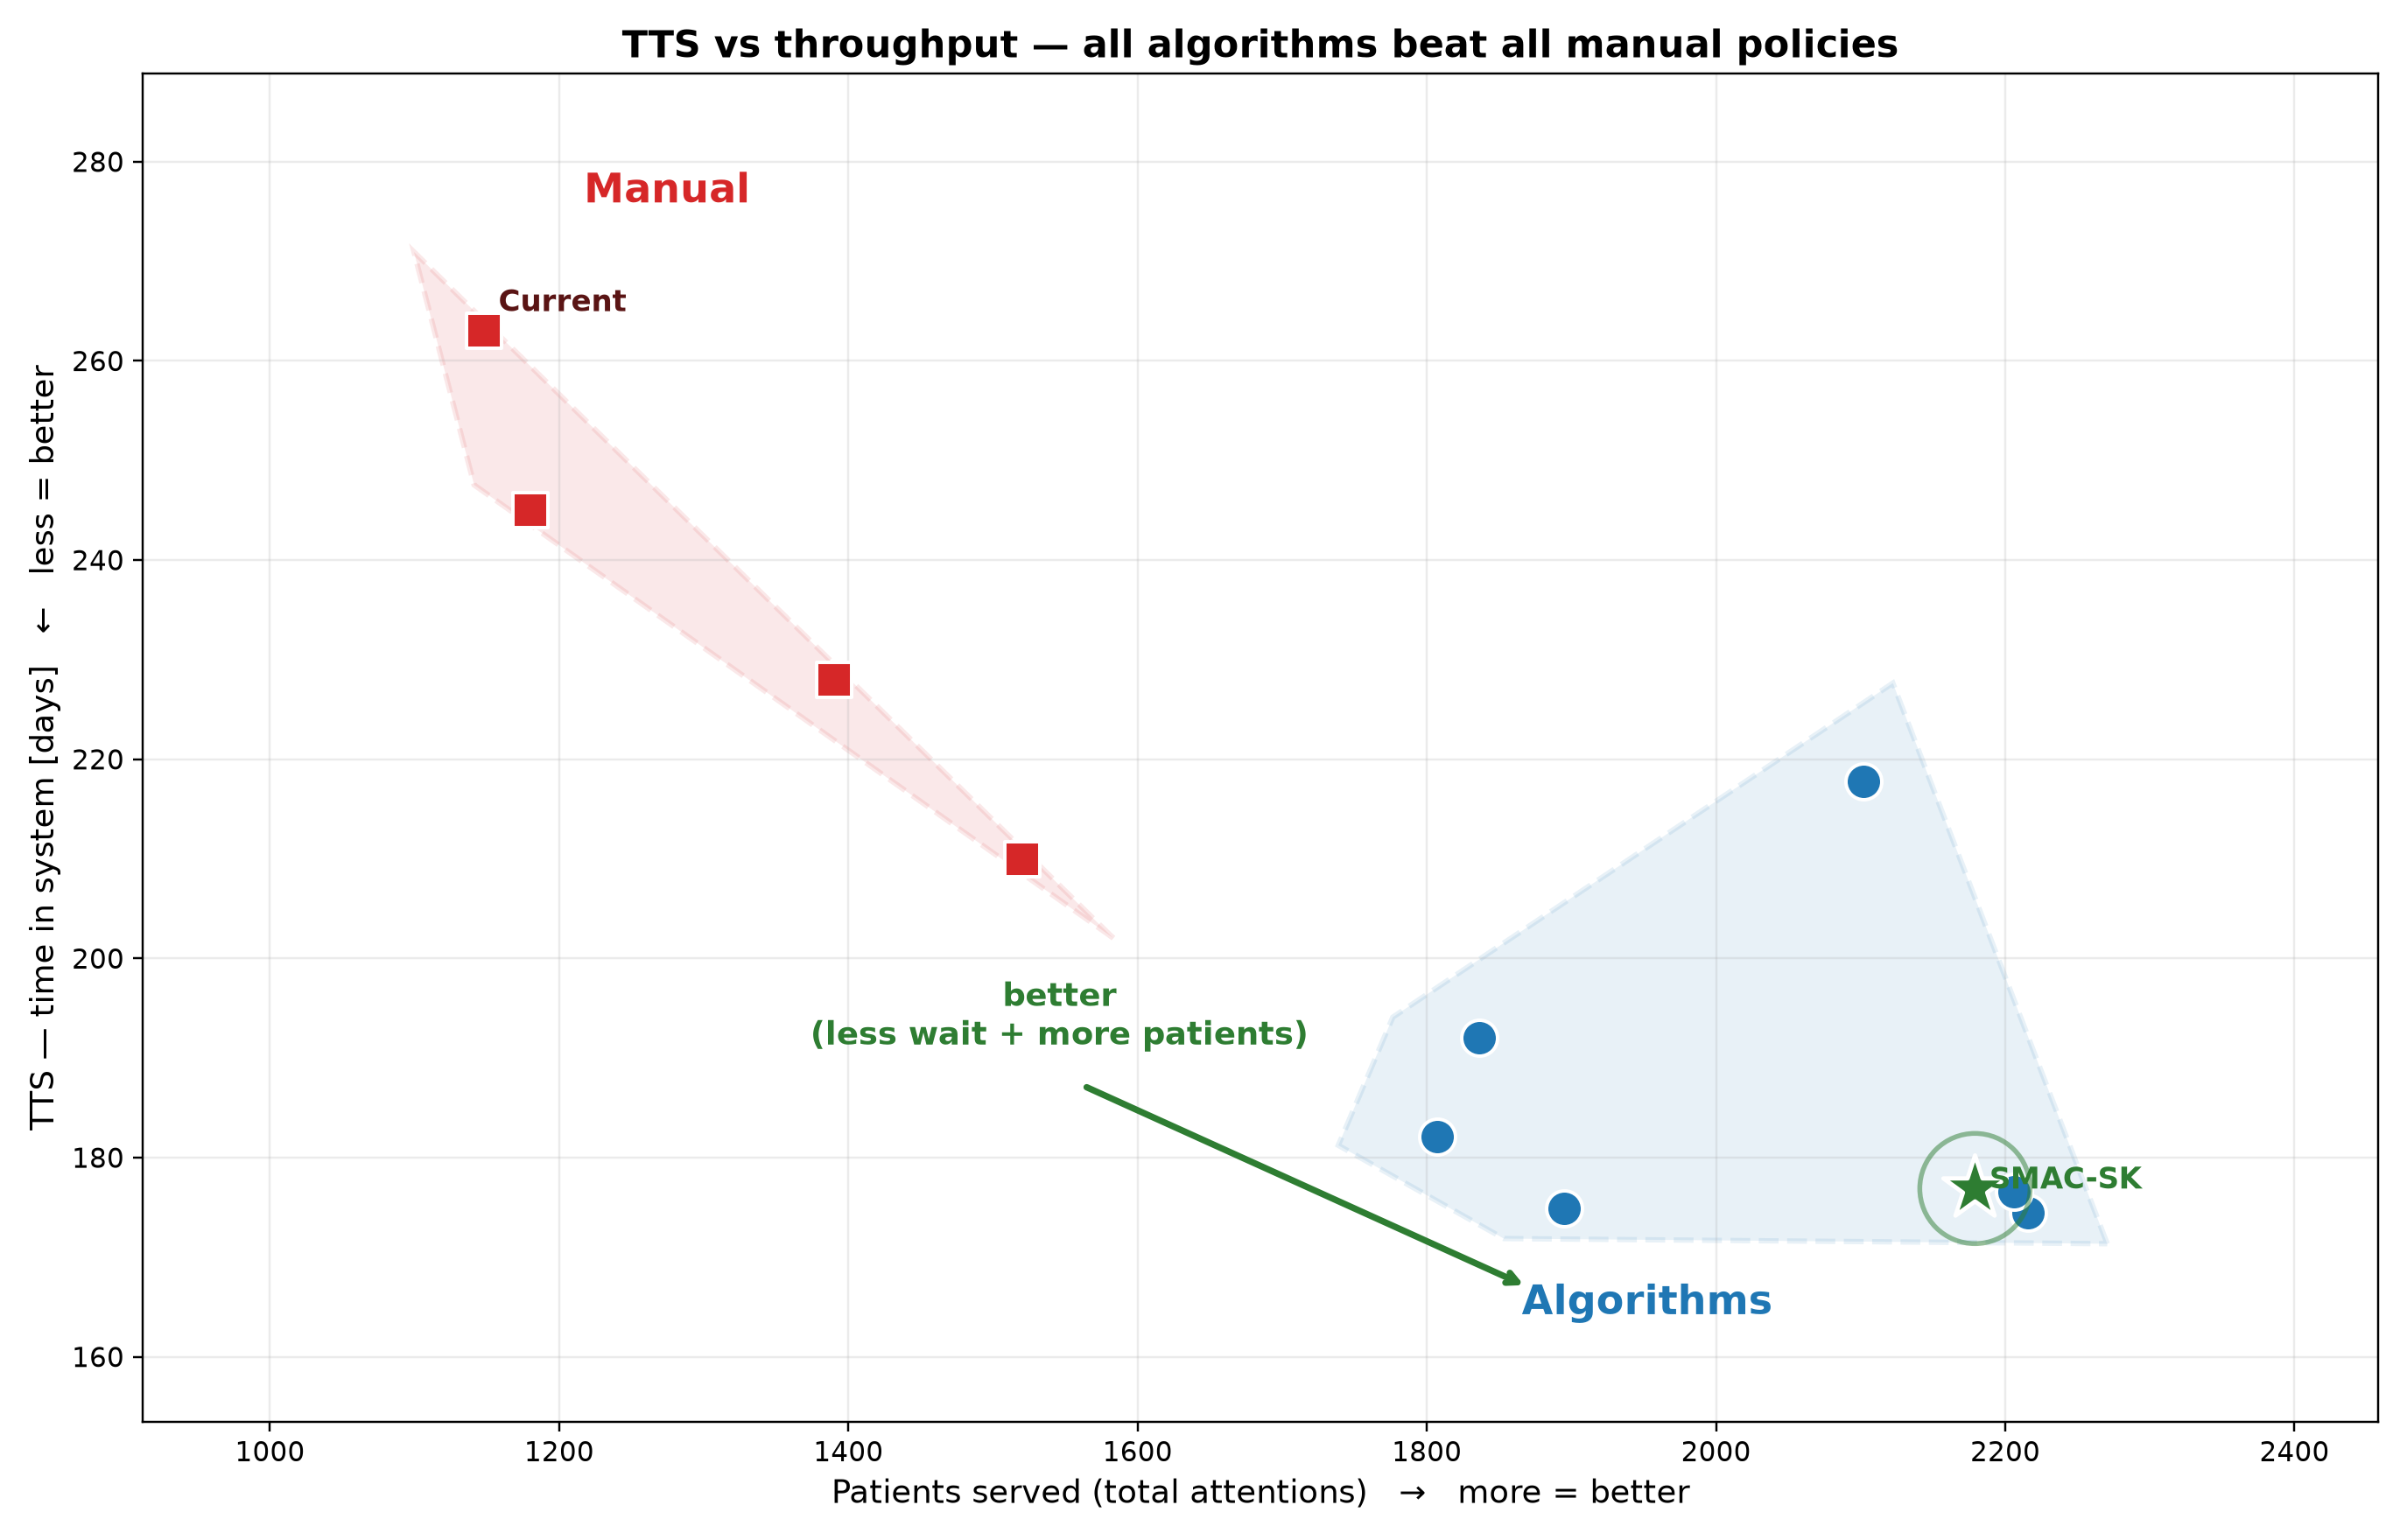
\includegraphics[width=\textwidth]{fig_pareto.png}
\caption{ATS vs.\ patients served for each benchmarked method
(mean $\pm\,\sigma$ across 15 seeds). Every optimised policy
dominates the incumbent on both criteria.}
\label{fig:Pareto}
\end{figure}


\section{Discussion and Limitations}
\label{sec:discussion}

\subsection{Convergence behaviour and computational cost}

Figure~\ref{fig:convergence} tracks the best objective found against simulator evaluations and wall-clock compute time. SMAC-SK and SK-Adaptive improve quickly from the first evaluations and track closely throughout the search. SPSA is more erratic early on, reflecting its single-random-direction gradient estimate, but converges to a comparable final value. ASTRO-DF covers a visibly narrower range of evaluations under the same nominal budget because its adaptive-sampling criterion accumulates replications at each point rather than exploring the space; Figure~\ref{fig:exectime} shows it requires three to four times the wall-clock time per seed of every other method. The shared evaluation budget therefore buys ASTRO-DF substantially less real search, which reframes the result in Table~\ref{tab:results}: its formal almost-sure convergence guarantee does not translate into competitive performance within a fixed compute envelope when the noise assumption underlying that guarantee is violated. Among surrogate-based methods, SMAC-RF is the slowest to approach its final value by compute time, consistent with random forests requiring more retraining overhead as the evaluated dataset grows.

\begin{figure}[H]
\centering
\includegraphics[width=\textwidth]{conv.png}
\caption{Algorithm convergence (mean $\pm\,\sigma$ across seeds), by number of simulator
evaluations (left) and by wall-clock compute time (right). ASTRO-DF is omitted from
the compute-time panel because its per-seed runtime (Appendix~\ref{app:time}) falls
far outside the range shown.}
\label{fig:convergence}
\end{figure}

\begin{figure}[H]
\centering
\includegraphics[width=0.75\textwidth]{time.png}
\caption{Execution time per seed, by method.}
\label{fig:exectime}
\end{figure}

\subsection{Managerial implications}

The optimised configurations converge on a consistent qualitative prescription relative to the incumbent policy and two intermediate expert-driven policies (``Management'' and ``Mgmt+Cap'', which adjust only slot counts and staffing): every optimizer-found configuration drives first-consultation blocking, empty-consultation, non-contactability, and post-control blocking rates to approximately 5\%, uniformly, versus 10--34\% under the expert-driven policies. Administrative tightening — not only the addition of slots, diagnostic capacity, and staff — is where a large share of the improvement originates. A policy that adds capacity without correcting blocking and non-contactability rates captures only part of the available gain. For a decision-maker at CRS Cordillera, the prescription is specific and auditable: modest capacity increases combined with a disciplined reduction of scheduling and follow-up slack.

\begin{figure}[H]
\centering
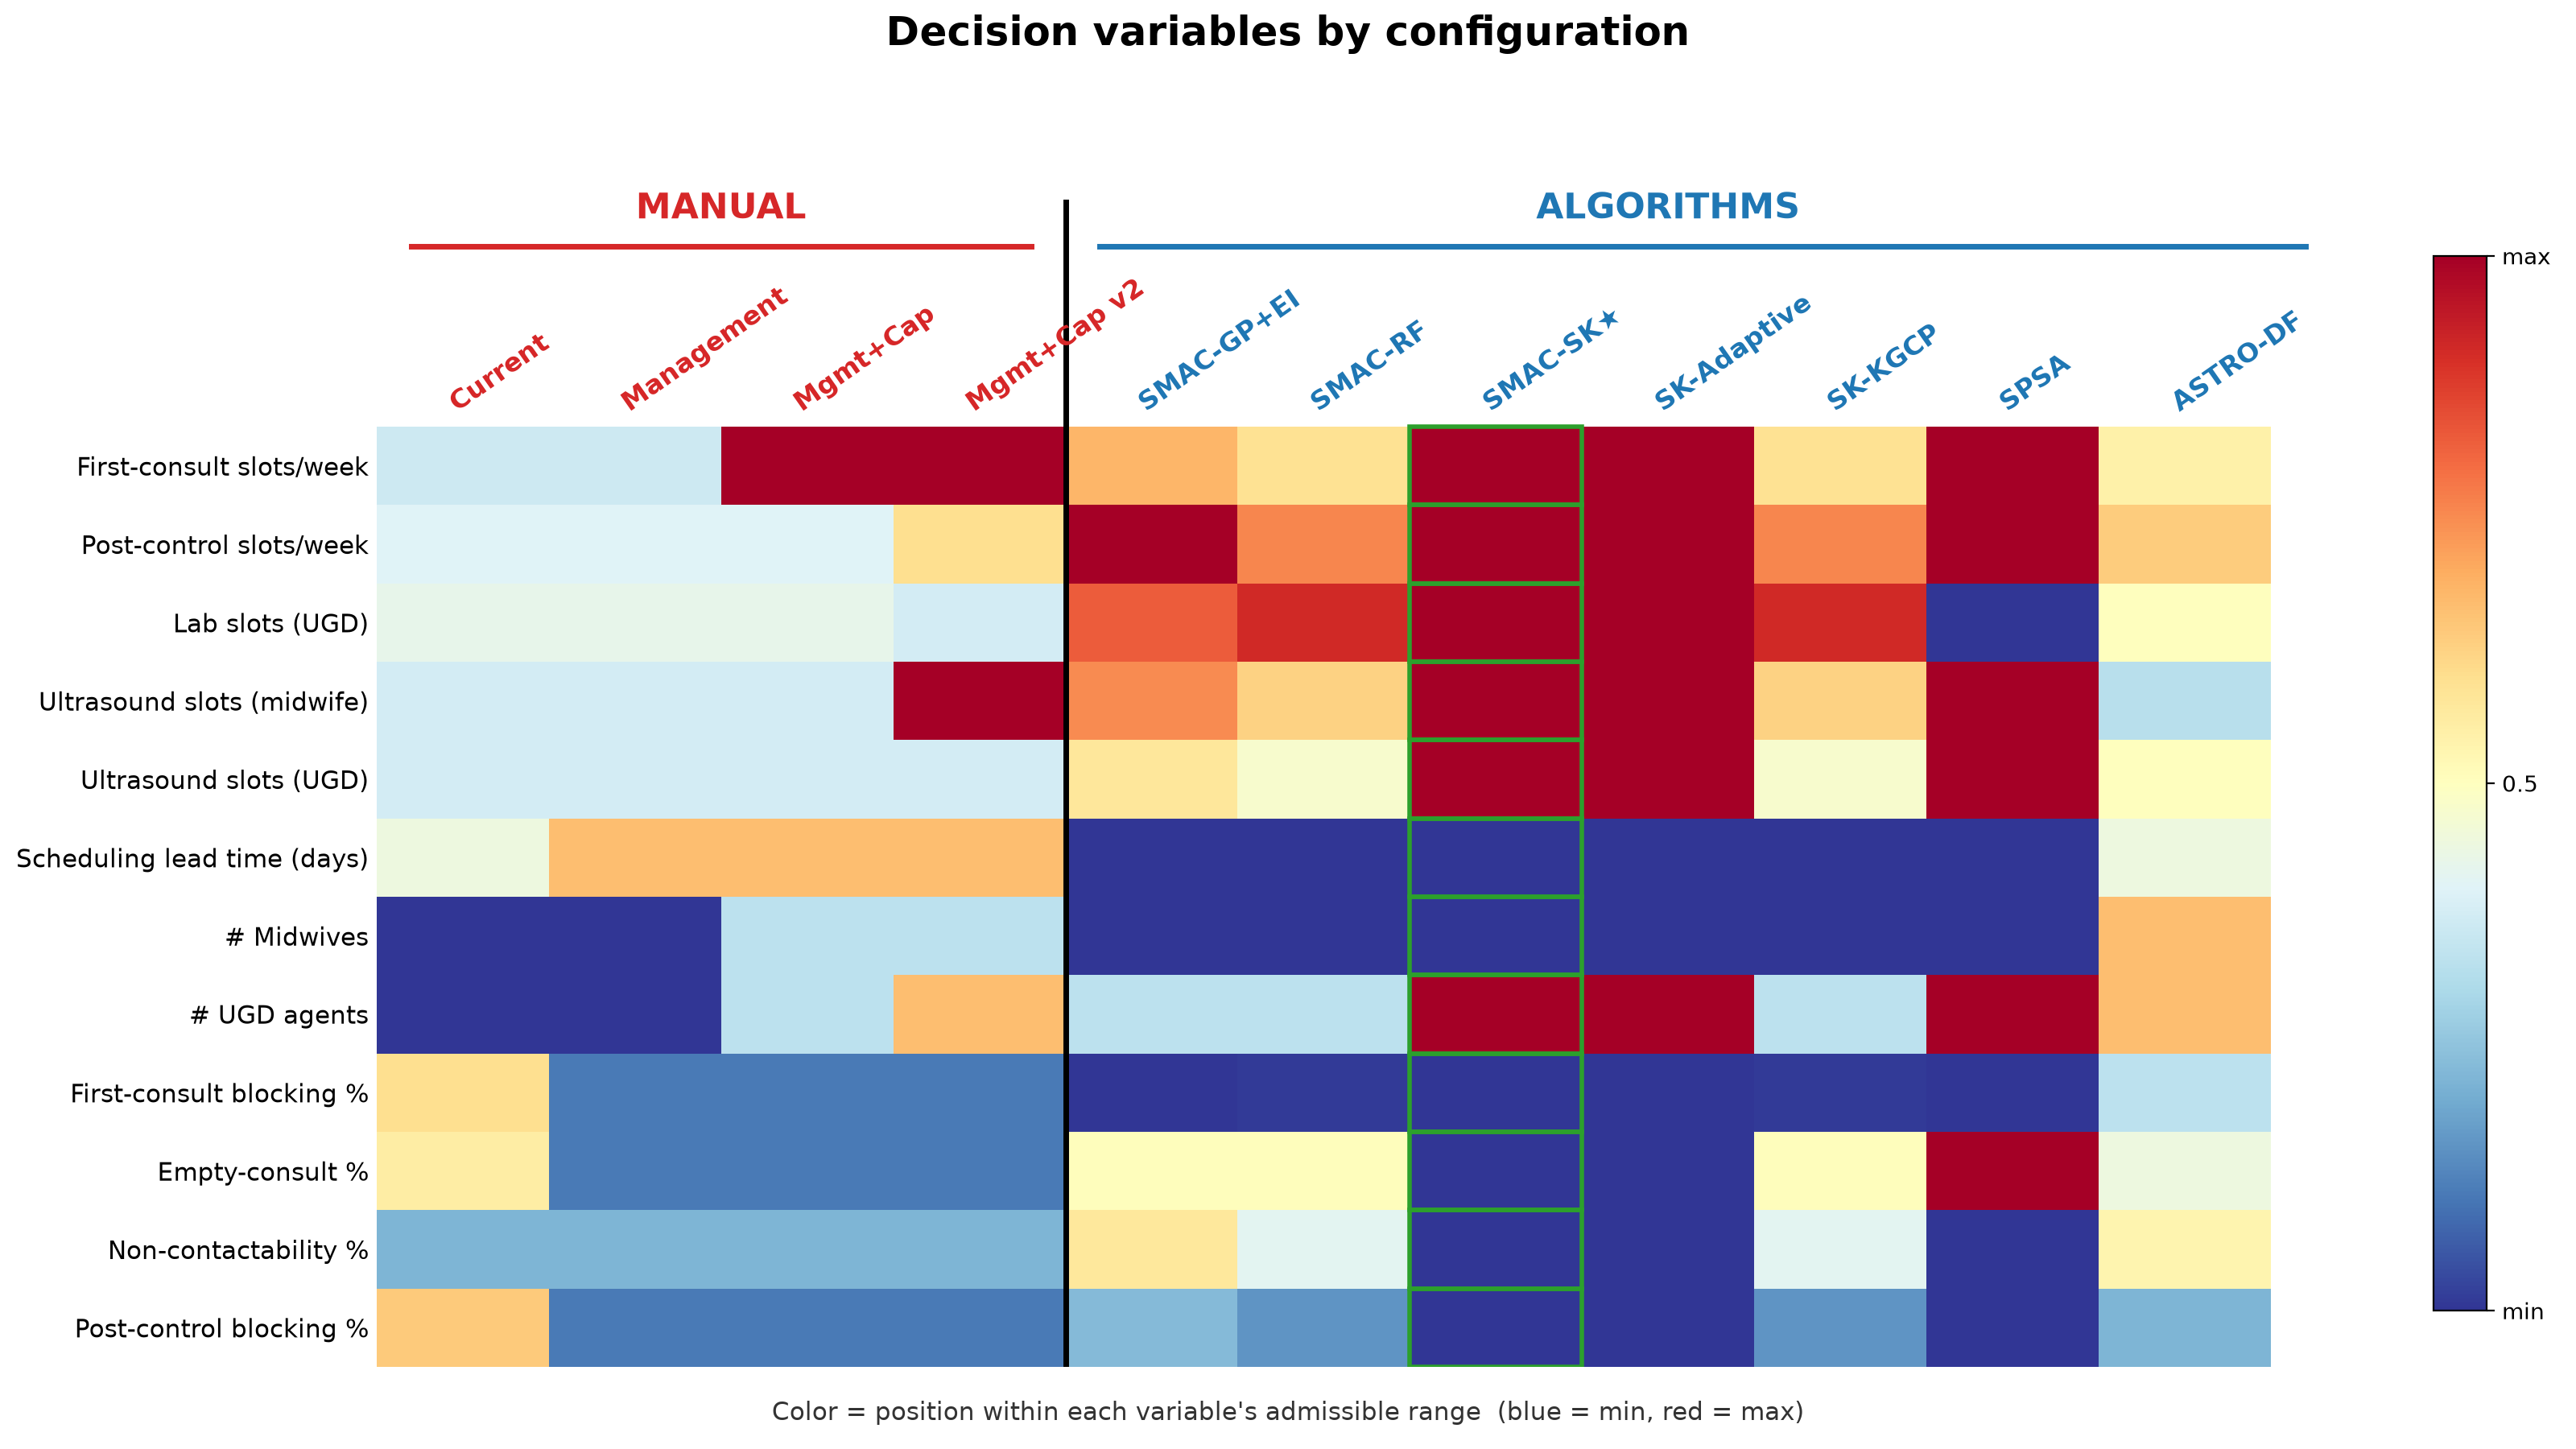
\includegraphics[width=\textwidth]{fig_variables_heatmapv2.png}
\caption{Decision variables by configuration: expert-driven policies (left of vertical
line) versus optimizer-found configurations (right). Cell colour indicates each
variable's normalised position within its admissible range (white = minimum,
dark red = maximum); administrative-rate variables (lower four rows) converge
near the minimum across all optimised configurations.}
\label{fig:decisionvars}
\end{figure}

\subsection{Limitations}

The study has one limitation that bounds the scope of its conclusions. The DES evaluator and benchmark results are specific to CMI at CRS Cordillera. The decision-variable structure is generic to ambulatory specialty care, but transferability to another clinic or specialty within the SSMO network has not been tested empirically.


\section{Conclusions and Future Work}
\label{sec:conclusions}

Every algorithm evaluated reduces ATS by 27--34\% relative to the incumbent policy while simultaneously increasing patients served — a strict Pareto improvement with no wait-time/throughput trade-off. The central contribution is applied: SMAC-SK, obtained by replacing SMAC's default surrogate with a stochastic-kriging model, is a practical and effective tool for prescriptive capacity planning in this setting. Its explicit decomposition of intrinsic simulation variance and extrinsic metamodel uncertainty lets the acquisition function distinguish configurations that need more replications from those that need more exploration — a distinction the evaluator's structural heteroscedasticity makes necessary. Empirically, SMAC-SK attains a reduction statistically indistinguishable from the best point estimate (SPSA) while achieving the tightest confidence interval among competitive methods, the property that matters when a configuration is deployed once and not re-tuned.

A second finding concerns the relationship between formal convergence guarantees and achieved performance. ASTRO-DF — the only benchmarked method with a proven almost-sure convergence guarantee — yields the worst mean result and the highest computational cost per seed. The guarantee rests on a homoscedastic noise assumption that the DES evaluator violates structurally, and the adaptive-sampling criterion responds by accumulating replications rather than exploring the space. The practical implication is that a convergence guarantee calibrated for homoscedastic noise does not translate into competitive performance within a fixed compute envelope when that assumption fails.

No existing method natively combines structural heteroscedasticity, mixed-integer decision variables, and formal convergence guarantees. Future work targets a mixed-integer DFO method with adaptive replication allocation driven by local variance estimation, and the regularity conditions under which almost-sure convergence to first-order stationary points can be established for this class of evaluator. Empirical extensions should address transferability beyond the single site studied here and joint optimisation of wait-time outcomes with staff workload.


\section*{Acknowledgments}
This research was partially funded by Fondecyt Regular Grant 1231245 and by a VRIP doctoral scholarship, Pontificia Universidad Cat\'olica de Chile. We thank the CRS Cordillera and Servicio de Salud Metropolitano Oriente teams for access to operational data.


\appendix

\section{Replication budget}
\label{app:replication}
\begin{table}[H]
\centering
\caption{Replication-budget analysis for the ATS key performance indicator.}
\begin{threeparttable}
\begin{tabular}{@{}llcccr@{}}
\toprule
Method & Criterion & Est.\ mean & Std.\ dev. & 95\% CI & Rec.\ runs \\
\midrule
Method 1 & Abs.\ error $\pm5$ days & 260.51 & 9.30 & [253.9, 267.2] & 18 \\
Method 2 & Rel.\ error 5\%         & 260.51 & 9.30 & [253.9, 267.2] & 10 \\
Method 3 & Seq., rel.\ error 5\%   & 262.25 & 14.65 & [250.0, 274.5] &  8 \\
\bottomrule
\end{tabular}
\begin{tablenotes}
\footnotesize
\item KPI = ATS, mean patient time in system (days).
\end{tablenotes}
\end{threeparttable}
\end{table}

\section{Statistical validation of the DES model}
\label{app:validation}
\begin{table}[H]
\centering
\caption{Mann--Whitney $U$ test: simulated vs.\ real first-consultation
         waiting times.}
\label{tab:validation}
\begin{tabular}{@{}ll@{}}
\toprule
Test      & Mann--Whitney $U$ (two-sided, $\alpha=0.05$) \\
$H_0$     & Simulated $\overset{d}{=}$ Real data \\
Statistic & $U = 865{,}529$ \\
$p$-value & $0.0564$ \\
Decision  & Fail to reject $H_0$ \\
\bottomrule
\end{tabular}
\end{table}

\section{Execution time by method}
\label{app:time}
Figure~\ref{fig:exectime} reports wall-clock execution time per seed for each of the
seven optimizers under the shared evaluation budget described in
Section~\ref{sec:method}. Six methods (SMAC-SK, SK-KGCP, SPSA, SMAC-GP+EI,
SK-Adaptive, SMAC-RF) fall within a broadly similar range, with medians from
approximately 17 to 25 hours per seed; ASTRO-DF is a clear outlier at approximately
67--73 hours per seed, three to four times the cost of every other method.
ASTRO-DF's low output variance (Table~\ref{tab:results}) is therefore attained at
substantially higher computational cost, consistent with the convergence/performance/cost
trade-off discussed in Section~\ref{sec:discussion}.


\bibliographystyle{plainnat}
\bibliography{bibliography}

\end{document}
